%! Tex program = pdflatex
 
\documentclass[UTF8]{ctexart}
\CTEXsetup[format={\Large\bfseries}]{section}
\usepackage{amsmath}
\usepackage{ctex}
\usepackage{array}
\usepackage{ulem}
\usepackage{graphicx}
\usepackage{geometry}
\usepackage{multirow}
\usepackage{subfig}
\usepackage{float}
\usepackage{multicol}
\usepackage{multirow}
\usepackage{indentfirst}
\usepackage{makecell}
\geometry{papersize={21cm,29.7cm}}
\geometry{left=2.54cm,right=2.54cm,top=3.18cm,bottom=3.18cm}
\usepackage{fancyhdr}
\pagestyle{fancy}
\lhead{\today}
\chead{}
\rhead{2020011075}
\lfoot{清华大学}
\cfoot{\thepage}
\rfoot{物理实验B(1)}
\renewcommand{\headrulewidth}{0.4pt}
\renewcommand{\headwidth}{\textwidth}
\renewcommand{\footrulewidth}{0pt}
\usepackage{bm}
\begin{document}
\begin{titlepage}
    \begin{center}
		\quad \\
		\quad \\
        \quad \\
        \quad \\
        \quad \\
        \quad \\
		\kaishu \fontsize{30}{15} 直流电桥测电阻实验报告

	\end{center}
	\vskip 10cm

    \begin{center}
        \begin{large}
        \begin{tabular}{cc}
        院\qquad 系:& ~~~~~~~~自动化系~~~~~~~~      \\
        \cline{2-2}\\
        班\qquad 级:& 自02班   \\
        \cline{2-2}\\
        学生姓名:& 彭程    \\
        \cline{2-2}\\
        学\qquad 号:&2020011075   \\
        \cline{2-2}\\
        组\qquad 号:& 单一晚M    \\
        \cline{2-2}\\
        座~~位~~号:& \# 13    \\
        \cline{2-2}
        \end{tabular}
        \end{large}
        \end{center}

\end{titlepage}
\newpage
\tableofcontents
\newpage
\section{实验名称}
直流电桥测电阻
\section{实验目的}
\begin{enumerate}
\item 了解单电桥测电阻的原理,掌握直流单桥使用方法;
\item 单电桥测量铜丝的电阻温度系数,学习用作图法和直线拟合法处理数据;
\item 构造非平衡互易桥组装数字温度计,学习桥路的应用分析设计;
\item 了解双电桥测量低电阻的原理,初步掌握双电桥的使用方法。
\end{enumerate}
\section{实验原理}
    \subsection{惠斯通电桥测电阻} 
    惠斯通电桥 (单电桥)电路原理如图1所示:
    
    \begin{figure}[ht]
        \centering
        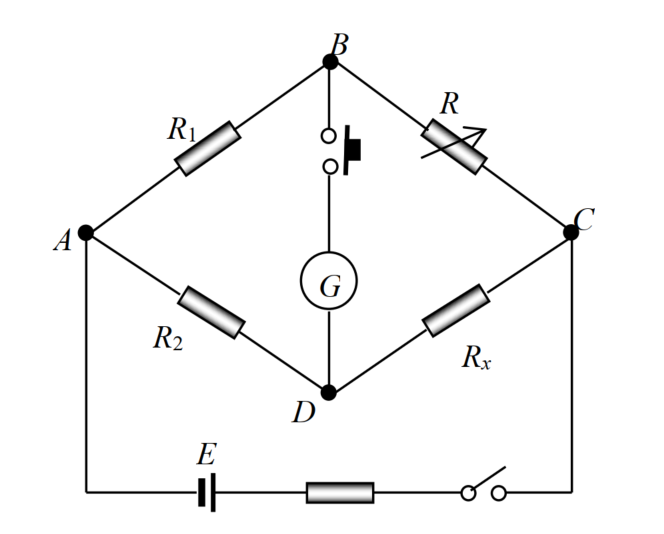
\includegraphics[scale=0.5]{惠斯通电桥.png}
        \caption{惠斯通电桥电路图}
        \label{fig:label}
    \end{figure}
    

    图中$R_{1}$、$R_{2}$ 和$R$阻值已知,
    与被测电阻$R_{x}$连成四边形, 每条边为电桥的一个臂。对角$A$和$C$之间接电源E;
    对角$B$和$D$之间接有检流计$G$ , 即为“桥”。当$B$ 、$D$电位相等时,
    桥路检流计$G$中无电流通过(故检流计又称为指零仪),即电桥达到了平衡。此时有:
    $$
        \frac{R_{x}}{R_{2}}  = \frac{R}{R_{1}}
    $$

    也即:
    \begin{align}
        R_{x}=\frac{R_{2}}{R_{1}} R
    \end{align}

    检流计足够灵敏时能相当好地成立,$Rx$就能用三个标准电阻的值来求得,而与电源电压无关。
    从而测量的准确度较高。

    单电桥的实际电路如图2所示: 

    \begin{figure}[h]
        \centering
        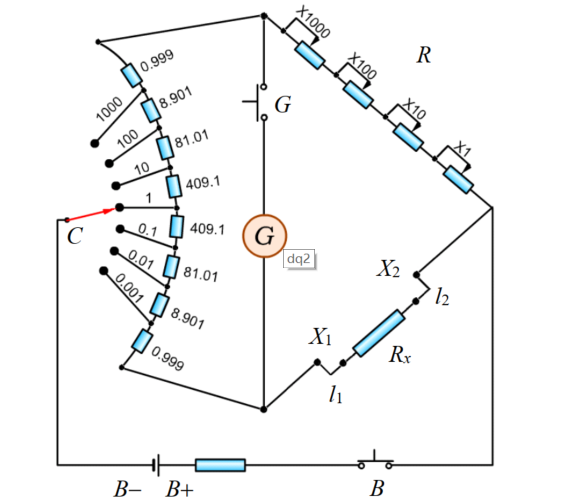
\includegraphics[scale=0.5]{单电桥.png}
        \caption{单电桥电路图}
        \label{fig:label}
    \end{figure}

    将$R_2$和$R_1$做成比值为$C$的比率臂,则被测电阻为:
    $Rx = CR$。

    将检流计灵敏阈(0.2 分格)所对应的被测电阻的变化量$\Delta s$ 叫做电桥的灵敏阈,有:
    
    \begin{eqnarray}
        \Delta_{s} & = & 0.2 C \frac{\Delta R}{\Delta d}
    \end{eqnarray}

    电桥的灵敏域越大,电桥越不灵敏。

    \subsection{双电桥测低电阻}

    为减小附加电阻的影响,在双电桥中作了两处改进:

    \begin{figure}[htbp]
        \begin{minipage}[t]{0.45\linewidth}
        \centering
        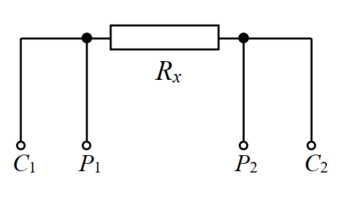
\includegraphics[scale=0.6]{低电阻四端接法.png}
        \caption{低电阻四端接法}
        \end{minipage}%
        \begin{minipage}[t]{0.45\linewidth}
        \centering
        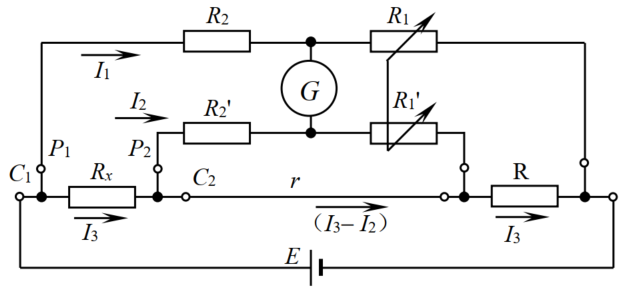
\includegraphics[scale=0.6]{双电桥原理图.png}
        \caption{双电桥电路}
        \end{minipage}
    \end{figure}

    (1) 被测电阻和测量盘电阻均采用四端接法,从而减小附加电阻的影响。

    (2) 电路中增设了两个臂𝑅1′和𝑅2′(如图 4 所示),其阻值较高。流过检流计 G 的电流为零时,电桥达
    到平衡,根据电路平衡条件可以推导出:

    \begin{eqnarray}
        R_{x} & = & \frac{R_{2}}{R_{1}} R+\frac{R_{1}^{\prime} r}{R_{1}^{\prime}+R_{2}^{\prime}+r}\left(\frac{R_{2}}{R_{1}}-\frac{R_{2}^{\prime}}{R_{1}^{\prime}}\right)
    \end{eqnarray}

    设计上尽量使$R_{2} / R_{1}=R_{2}^{\prime} / R_{1}^{\prime}$,并且用粗铜导线连接减小电阻,因此:
    $$ R_{x}=\frac{R_{2}}{R_{1}} R$$

    \subsection{铜丝的电阻温度特性以及数字温度仪的设计}
    \noindent (1) 铜丝的电阻温度特性

    多数金属的电阻随着温度的升高而增大:$R_{t} = R_{0}\left(1+\alpha_{R} t\right)$

    $R_{t}$ 、 $R_{0}$  分别是 $ t^{\circ} \mathrm{C}$ 、$ 0^{\circ} \mathrm{C}$  时金属的电阻值,于是有:
    \begin{eqnarray}
        \alpha_{R} & = & \frac{R_{t}-R_{0}}{R_{0} t}
    \end{eqnarray}

    \noindent (2) 铜电阻数字温度计设计

    根据铜的电阻系数,采用电桥,可制成数字温度计来测温。

    \noindent \textbf{非平衡电桥:}
 
    而非平衡电桥则是将平衡电桥的检流计G去掉,通过测量其两端的电压$U_t$来确定电阻,即:
    $$U_{t}=E\left(\frac{R_{1}}{R_{1}+R}-\frac{R_{2}}{R_{2}+R_{t}}\right)$$

    \noindent \textbf{互易桥:}

    将图 2 电桥线路中电源 $ E $ 和检流计 $ G $ 互易位置(电路与原来的等效), 
    $ R_{1}$ 、$ R_{2}$  分别和  $R $、$ R_{\mathrm{t}} $ 同数量级。
    将 $ G$ 换成 $ \mathrm{mV}$  表, 就改成互易了的非平衡桥, 用它测量  $U_{t}$  非线性误差会减小:
    \begin{eqnarray}
        U_{t} & = & E\left(\frac{R_{1}}{R_{1}+R_{2}}-\frac{R}{R+R_{t}}\right)
    \end{eqnarray}

    误差减小的原因见实验小结中预习思考题(5)的分析。


    \noindent \textbf{数字温度计线性化设计:}

    要求组装的温度计显示值与温度之间满足关系:
    \begin{eqnarray}
        U_{t} & = & \frac{1}{10} t(\mathrm{mV})
    \end{eqnarray}
    设温度  $t=0^{\circ} \mathrm{C} $ 时, $ U_{0}=0 \mathrm{mV} $时互易桥为平衡桥, 即有
    $ \frac{R_{2}}{R_{1}}= \frac{R_{0}}{R}=C $。
    故非平衡桥输出电压:
    \begin{eqnarray}
        U_{t} & = & E\left[\frac{1}{1+C}-\frac{1}{1+C\left(1+\alpha_{R} t\right)}\right] 
         =  E \frac{C \alpha_{R} t}{(1+C)^{2}} \cdot \frac{1}{1+\frac{C \alpha_{R}}{1+C} t}
    \end{eqnarray}
    实验中 $ \mathrm{C}=0.01<<1 $, 铜电阻温度系数  $\alpha_{R} \sim 10^{-3} \mathrm{C}^{-1} $, 则可近似为
    \begin{eqnarray}
        U_{t} & = & \frac{E C \alpha_{R}}{(1+C)^{2}} t+\Delta U
    \end{eqnarray}
    其中 $ \Delta U \approx-E \frac{\left(C \alpha_{R} t\right)^{2}}{(1+C)^{3}} $ 为非线性误差项可忽略, 则有
    
    \begin{eqnarray}
        E & = & \frac{(1+C)^{2}}{10 C \alpha_{R}}
        \end{eqnarray}
    至此已完成线性化设计,且有  $U_{t}=\frac{1}{10} t+\Delta U(\mathrm{mV}) $。



    

\section{实验仪器}
\noindent QJ-23型直流单电桥

\noindent 铜丝电阻温度系数测量装置(包括电加热器、温度计、直流电机、铜丝电阻、稳压电源、单电桥、搅拌器、水浴装置)

\noindent 数字调压器

\section{实验任务或步骤}

\subsection{惠斯通电桥测电阻}
\noindent(1) 熟悉电桥结构,预调检流计零位。\\
(2) 测不同量级的待测电阻值,并得到读数C和R的值同时计算灵敏阈。\\
(3) 根据记录的数据计算测量值$R_x$,分析误差,最后给出各电阻的测量结果。
\subsection{单电桥测铜丝的电阻温度系数}
\noindent(1) 测量加热前的起始水温及铜丝电阻值。\\
(2) 从起始温度开始升温,每隔$5\sim6^{\circ}C$左右测一次温度 $t$ 及相应的阻值 $R_t$。\\
(3) 在大致热平衡(温度计示值基本不变)时进行测量。\\
(4) 用计算机对{$t$}和{$R_t$}进行直线拟合,记录 a、 b 及相关系数 r,计算铜的电阻温度系数$\alpha_R$及
$0^{\circ}C$时的电阻 $R_0$。用作图法求$\alpha_R$代入相应公式计算$\alpha_R$。\\
\subsection{铜电阻数字温度计的设计组装与校验}

\noindent(1) 改单桥为互易非平衡桥;\\
(2) 选择设置桥 路参数  $C $、$ R$  及 $ E $;\\
(3) 每间隔 $ 4 \sim 5^{\circ} \mathrm{C}$  测一次  $U_{t} $ 和  $t$ , 测  $5 \sim 6$  组;\\
(4) 上机拟合, 检验 $ U_{t} \sim t$  的线性关系 $ U_{t}=a+b t $, 记录 $ a $、$ b$ 、 $r$  等。

\section{数据处理}
\subsection{惠斯通电桥测电阻}
\renewcommand\arraystretch{1.5}
\setlength{\tabcolsep}{3mm}{
\begin{tabular}{|l|c|c|c|c|}
    \hline 
    \multicolumn{1}{|c|}{ 电阻标称值($\Omega$)} &~~~~120~~~~~&~~~~1k~~~~&~~~~11k~~~~~&~~~~360k~~~~~\\
    \hline  \small 比率臂读数 C &0.1&0.1&10&100\\
    \hline  \small 准确度等级指数$ \alpha$ &0.2&0.2&0.2&0.2 \\
    \hline  \small 平衡时测量盘读数  $R(\Omega)$ &1193 &9890 &1099 &3632  \\
    \hline \makecell[l]{ \small 平衡后将检流计调偏\\\small $\Delta d$ (格)}  &3.0 &3.5 &2.1 &3.9  \\
    \hline \makecell[l]{ \small 与  $\Delta d $ 对应的测量盘\\\small 的示值变化 $\Delta R(\Omega)$} &2 &2 & 6& 1000 \\
    \hline  \small 测量值  $C R(\Omega)$ & 119.3&989.0 &10990 &362300  \\
    \hline \makecell[l]{ \small $\left|E_{\lim }\right|=(\alpha \%)(C R+500 C)(\Omega)$} &0.3368 &2.078 &31.98 &824.6 \\
    \hline \small$\Delta_{s}=0.2 C \Delta R / \Delta d(\Omega)$ &0.01333 &0.01143 &5.714 &5128  \\
    \hline \small$\Delta_{R_{x}}=\sqrt{E_{\lim }^{2}+\Delta_{S}^{2}}(\Omega)$ &0.3389 &2.078 &32.49 &5194  \\
    \hline \small$R_{x}=C R \pm \Delta_{R_{x}}(\Omega)$ &119.3$\pm$0.3398 &989.0$\pm$2.078 &10990$\pm$32.49 &362400$\pm$5194  \\
    \hline
\end{tabular}}

\makeatletter
\newcommand\dlmu[2][4cm]{\hskip1pt\underline{\hb@xt@ #1{\hss#2\hss}}\hskip3pt}
\makeatother

\subsection{单电桥测铜丝电阻系数}

\setlength{\tabcolsep}{2mm}{
\begin{tabular}{|c|c|c|c|c|c|c|c|c|c|c|}
    \hline & 1 &2&3&4&5&6&7&8&9&10 \\
    \hline 温度$/{ }^{\circ}\mathrm{C}$ &27.3 &32.8&38.2&43.4&48.9&53.6&59.1&64.6&69.1&73.6 \\
    \hline  比率臂C&0.01&0.01&0.01&0.01&0.01&0.01&0.01&0.01&0.01&0.01 \\
    \hline 测量盘读数 R$/ \Omega$&1718&1755&1790&1824&1862&1893&1930&1965&1993&2023\\
    \hline  $R_t=CR / \Omega$&17.18&17.55&17.90&18.24&18.62&18.93&19.30&19.65&19.93&20.23 \\
    \hline
\end{tabular}}
\\
接下来使用计算机通过最小二乘法拟合回归直线($y=a+bx$,其中y表示$R_t$,~x表示t):

$$
b=\frac{\sum_{i=1}^{n} x_{i} y_{i}-n \bar{x} \bar{y}}{\sum_{i=1}^{n} x_{i}^{2}-n \bar{x}^{2}} =0.06595
$$


$$
a=\overline{y}-b\overline{x} = 15.39
$$

$$
  r=\frac{\sum_{k=1}^n(x_i-\bar{x})
  (y_i-\bar{y})}
  {\sqrt{\sum_{k=1}^n(x_i-\bar{x})^2
  \sum_{k=1}^n(y_i-\bar{y})^2}}=0.9999
$$

\noindent 故拟合直线方程:$R_t=a+bt=15.39+0.06595t$
\\
根据电阻温度关系:$R_t=R_0(1+\alpha_R t )$可知,回归直线中$b=R_0\cdot\alpha_t $ , $a=R_0$,故:
$$
\alpha_R=\frac{b}{a}=4.285\times 10^{-3} /{ }^{\circ}\mathrm{C}^{-1}
$$
\\
故拟合结果如下:

$a=\dlmu[2cm]{15.39}$

$b=\dlmu[2cm]{0.06595}$

$r=\dlmu[2cm]{0.9999}$  

$\alpha_R=$\dlmu[2cm]{$4.285\times 10^{-3} $}$/{ }^{\circ}\mathrm{C}^{-1}$ 

拟合曲线如下:
\begin{figure}[ht]
    \centering
    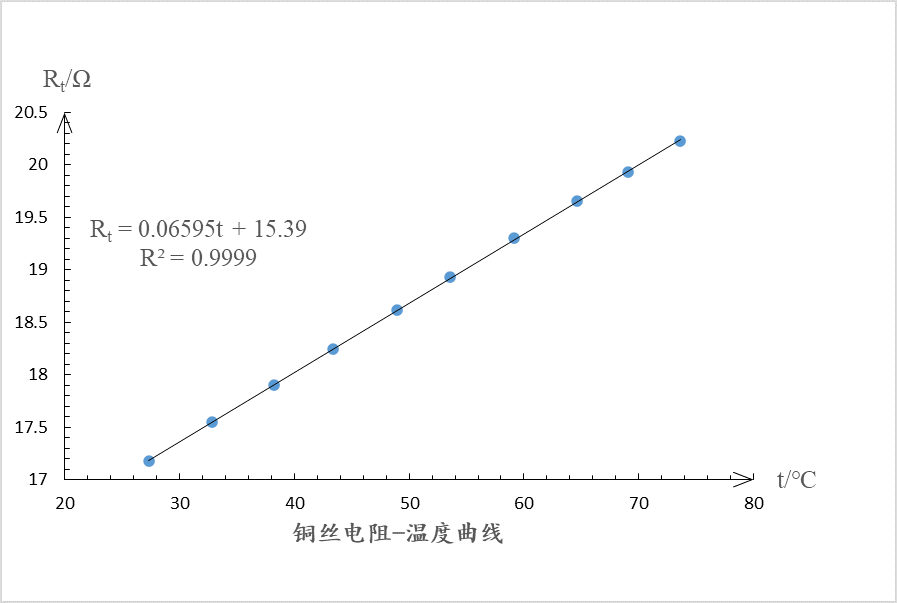
\includegraphics[scale=1]{铜丝电阻温度.png}
    \caption{铜丝电阻-温度特性曲线}
    \label{fig:label}
\end{figure}

使用绘图法绘图如图6所示
\begin{figure}[ht]
    \centering
    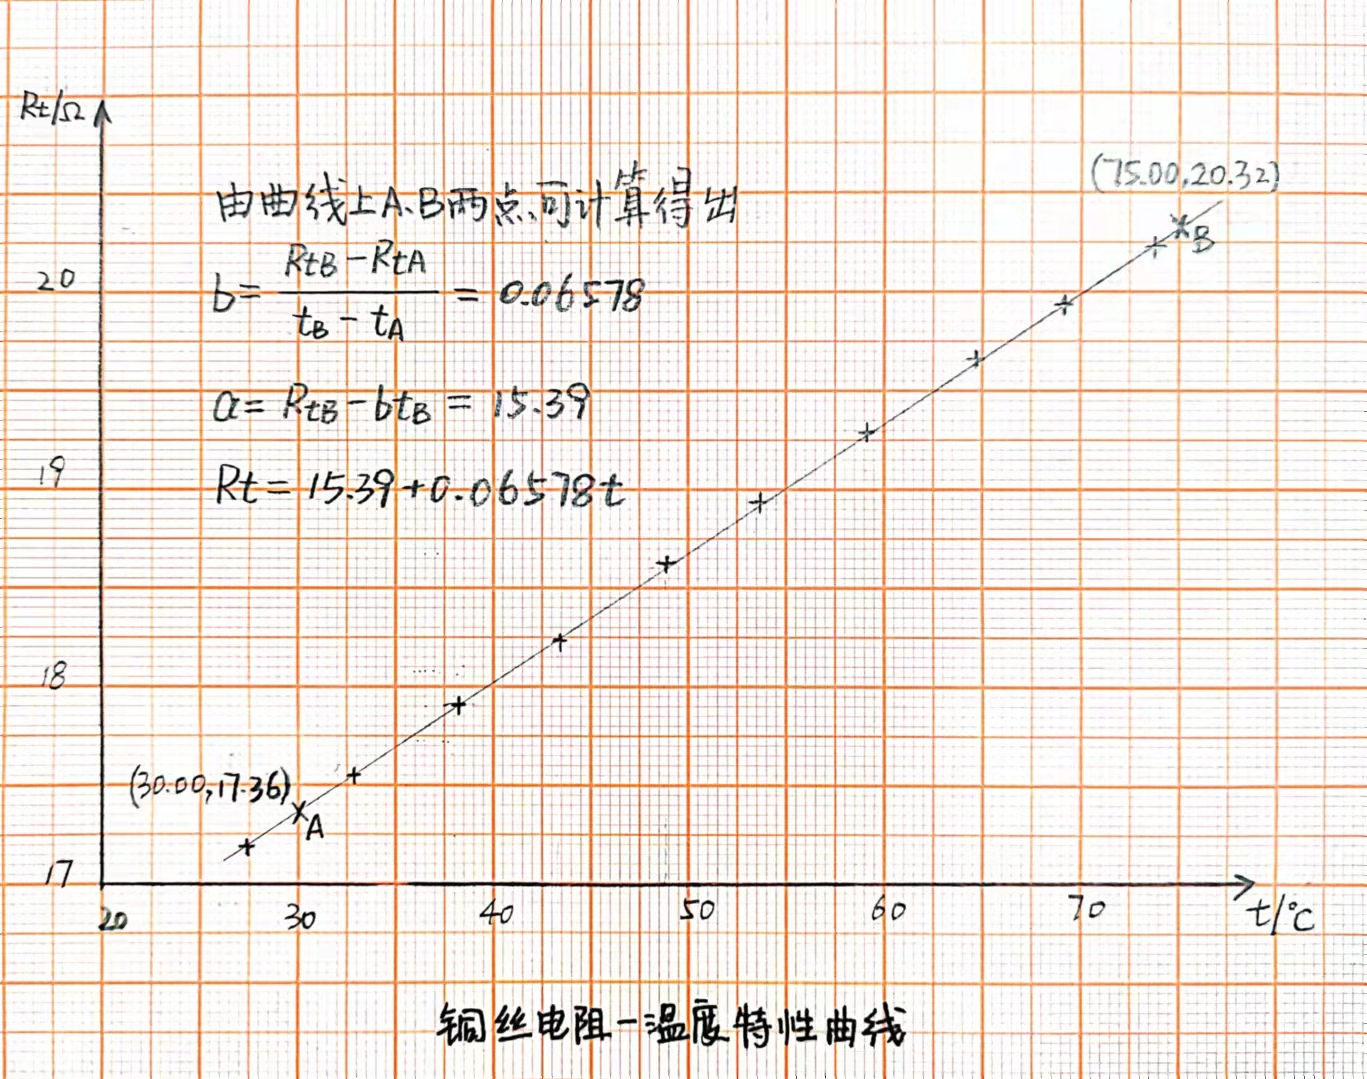
\includegraphics[scale=0.25]{手绘铜丝电阻温度.jpg}
    \caption{铜丝电阻-温度特性曲线(绘图法)}
    \label{fig:label}
\end{figure}

在绘图法绘出的曲线中取较远的两点$ (30.00,17.36)$,$(75.00,20.32)$,则有:
$$
b=\frac{R_{tB}-R_{tA}}{t_B-t_A}=0.06578
$$

$$
a=R_{tB}-b\cdot t_B= 15.39
$$

$$
R_t=15.39+0.06578t
$$

$$
\alpha_R=\frac{b}{a}=4.274\times 10^{-3}/{ }^{\circ}\mathrm{C}^{-1}
$$

对比两种方法得到的$\alpha_R$:计算机拟合得到的$\alpha_R=4.285\times 10^{-3} /{ }^{\circ}\mathrm{C}^{-1}$,
绘图法计算出的$\alpha_R=\frac{b}{a}=4.274\times 10^{-3}/{ }^{\circ}\mathrm{C}^{-1}$,两者差异很小,
说明测量和绘图比较准确。

\subsection{铜电阻数字温度计的设计组装及校验}
为组装温度与输出电压值近似满足关系$U_{t}=\frac{1}{10} t(\mathrm{mV}) $的温度计,设计过程如下:\\

由实验原理中的推导部分可知:
$$
    U_{t}  = \frac{E C \alpha_{R}}{(1+C)^{2}} t+\Delta U 
$$

忽略非线性误差项$\Delta U$后我们可以得到:
\begin{align}
    E & =  \frac{(1+C)^{2}}{10 C \alpha_{R}} \times 10^{3} \nonumber\\
    &\approx\frac{10}{ \alpha_{R}}\nonumber\\
    &=2.333 V\nonumber\\
\end{align}

温度为$0^{\circ}C$时电桥平衡,有$\frac{R_{0}}{R}=C $,故:
$$
R=100R_0=1539\Omega
$$

故温度计参数选取如下:

电源$E=\dlmu[1cm]{2.333}V$

电阻系数$\alpha_R=$\dlmu[2cm]{$4.285\times 10^{-3} $}$/{ }^{\circ}\mathrm{C}^{-1}$ 

比率臂 $ C=\dlmu[1cm]{0.01}$  

测量盘读数  $R =\dlmu[1cm]{1539} \Omega$

测量结果如下表所示:

\setlength{\tabcolsep}{5mm}{
\begin{tabular}{|c|c|c|c|c|c|c|c|}
    \hline & 1  &2&3&4&5&6&7 \\
    \hline 温度$/{ }^{\circ}\mathrm{C}$ &40.2 &46.7&52.4&57.9&63.2&66.4&69.0 \\
    \hline  $U_t / V$&4.02 &4.59&5.18&5.75&6.27&6.59&6.84 \\
    \hline
\end{tabular}}

接下来使用计算机通过最小二乘法拟合回归直线($y=a+bx$,其中y表示$U_t$,~x表示t):

$$
b=\frac{\sum_{i=1}^{n} x_{i} y_{i}-n \bar{x} \bar{y}}{\sum_{i=1}^{n} x_{i}^{2}-n \bar{x}^{2}} =0.09931
$$


$$
a=\overline{y}-a\overline{x} = -8.302\times10^{-3}
$$

$$
  r=\frac{\sum_{k=1}^n(x_i-\bar{x})
  (y_i-\bar{y})}
  {\sqrt{\sum_{k=1}^n(x_i-\bar{x})^2
  \sum_{k=1}^n(y_i-\bar{y})^2}}=0.9998
$$


其中a的结果很接近0.1,基本满足了我们$U_{t}=\frac{1}{10} t(\mathrm{mV}) $的设计需求;而b的值很小,符合其二阶小量的身份;同时相关系数接近1,表明温度计实现比较成功。

拟合曲线如下:
\begin{figure}[ht]
    \centering
    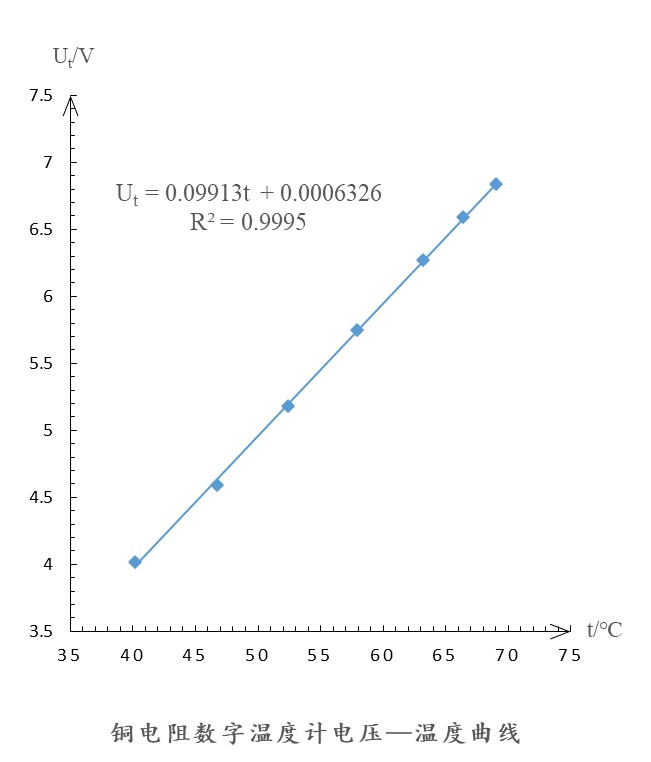
\includegraphics[scale=0.7]{温度计电压温度曲线.jpg}
    \caption{温度计电压-温度曲线}
    \label{fig:label}
\end{figure}


\section{实验小结}
\noindent  \textbf{预习思考题:}\\

\noindent  \textbf{(1)从原理上讲,惠斯通电桥主要是由哪几部分组成的? 电桥的平衡条件是什么?}

惠斯通电桥由四条桥臂、电源、检流计组成;电桥平衡的条件是检流计两端电位相等使得检流计没有电流通过。

\noindent  \textbf{(2)电桥法测量电阻是一种比较精确的方法,在测量前最好先用其它方法(如万用表)粗略测量被测电
阻的大小,这样做的目的是什么?}

预先知道待测电阻的大概阻值有助于快速选取合适的比率臂和测量臂。

\noindent  \textbf{(3)用惠斯通电桥测量电阻时,应如何正确使用电源按键开关B和检流计按键开关G?}

这两个按钮在测量时需要采用点按的方式,不可以长时间按下或者自锁;总开关B长时间连通会因为给电桥长时间通电产生的
电流热效应引起电路中电阻值的改变,检流计开关G的长时间连通会导致过载而烧坏检流计。只有在确保了通过检流计的电流很小的时候
才可以长时间按下G或者将其自锁以便于其他精确调节。

\noindent  \textbf{(4) 选择电桥比率臂的目的和原则是什么?}

目的是测量待测电阻的阻值;原则是比率臂比率应该使测量待测电阻时尽量用到测量臂千位盘。

\noindent  \textbf{(5) 在惠斯通电桥中将电源和检流计的位置互换,从理论上讲是否还可以测量电阻?对测量结果是否有
影响?}

理论上来说可以测量电阻,电桥的结构并没有发生本质变化,互易前后的连接方式是高度对称且等效的;在实际测量中会影响到测量的精度和误差,
原因是:当比率臂选取得较大或者较小时,两条支路的电阻差异大导致电流差异大,电阻较小的支路中任一个电阻发生
较小变化时会导致检流计两端电压发生较大变化,因而会导致测量结果的不准确甚至烧坏检流计,此时可以采用互易连接法交换电源和检流计的位置,
可以达到更好的检测效果和更小的误差。\\


\noindent  \textbf{课后思考题:}\\

\noindent  \textbf{(1) 为什么用单电桥测电阻一般比伏安法测量的准确度高?
单电桥中检流计的准确度对实验中所用的平衡电桥法测量有无影响?}

因为当检流计足够灵敏时,等式$R_x=\frac{R_2}{R_1} R$就能想到好地成立,
此时,待测电阻的阻值就可以用三个已知阻值的标准电阻表示出来,使得测量结果可以达到已知标准电阻
所具有的测量精度,与伏安法相比这一测量方式与电源电压、内阻、电压表、电流表的阻值无关,因而准确性更高。

由于检流计是否偏转是判断电桥是否平衡的唯一标准,所以检流计的准确度和灵敏度
对平衡电桥法测量电阻有着重大影响。



\noindent  \textbf{(2) 如果用实验中所用到的单电桥测一微安表的内阻,应怎样才能保证被测微安表不超量程?}

可以使用较高的比率臂,这样使得和待测微安表串联的$R_2$阻值很大,
使得微安表和一个大电阻串联减小了电流,
同时还可以在不影响实验测量精度的情况下减小电源电压,也可以起到减小电流的作用。
这样可以保证被测微安表不超过量程。


\noindent  \textbf{(3) 用电桥测量电感线圈的直流电阻时,为防止通断瞬间产生大电流损伤检流计或干扰测量,接通时应
先按合 B、后按合 G,断开时应先断 G 后断 B,为什么?}

因为电路中有电感线圈时,在电路通、断瞬间,电感上将产生比较大的电动势,如果先接通检流计再接通电源,
或者先断开电源再断开检流计,那么通断瞬间大电动势加在检流计两端就会产生很大的感应电流,从而烧坏检流计或干扰测量。
所以接通时应先按合 B、后按合 G,断开时应先断 G 后断 B。

\noindent  \textbf{(4) 直流双电桥和单电桥在结构上有什么不同?为什么前者适合于低值电阻的测量?}

双电桥被测电阻和测量盘均采用四端接法,且增设了两个阻值较高的臂$R_1'$,$R_2'$。

因为测量低电阻时,被测臂上有引线电阻和接触电阻,由于测量的是低电阻,故引线电阻和接触电阻不可忽略。
此时如果使用单电桥测电阻就会造成很大的误差。
而使用双电桥时,待测电阻和测量盘电压端的附加电阻和高阻值臂串联,其影响变小了,
两个电流端的附加电阻和导线串联,由计算表达式可知对结果并无影响,因此双电桥
将附加电阻带来的影响大大降低,从而适合于低阻值电阻的测量。



\noindent  \textbf{(5) 用惠斯通电桥测量电阻时,如果发现检流计的指针总是向一边偏转,请分析可能的原因。}

可能原因有:

检流计损坏;

检流计没有机械调零;

电阻盘R始终过大或者过小;

比率臂选择不合适。\\

\noindent  \textbf{总结:}\\

通过直流电桥测电阻的实验,我了解到了电桥测电阻的根本原理,
了解到了其误差的主要来源是检流计的灵敏度和附加电阻,知晓了金属电阻随温度变化的特性,掌握了测量了电阻温度系数的方法,
深入理解了数字温度计的设计原理并进行了实践。

对于检流计的灵敏度问题,我们可以采用适当提高电源电压的方式提高灵敏度;而对于附加电阻带来的误差,
我们可以使用双电桥的方式解决问题,通过通过四端接法和大电阻串联降低附加电阻带来的影响。

电阻温度系数随温度变化而变化,因为纯铜材料的温度系数在实验温度范围内变化很小故将其当做常量;在测量电阻温度系数时,
我们采用非平衡电桥和互易桥的方式来测量,其中非平衡电桥多用于非电量的电测量和生产过程的检测,
采用毫伏表替代检流计的作用,在实际应用中可以防止略大的导通电流带来的微安表的损坏,
同时非平衡桥的读数方便,可以快速、连续测量,这实现了“实时”地把该值转化为其他间接测量的物理量的设计要求。
而互易桥的引入一方面并没有改变电路的根本结构和测量关系,另一方面解决了两支路电阻差异大带来的可能的误差问题,
这启示我们要对原有方案加以改进从而在不改变实验原有思路的前提下改进实验。

电桥除了应用于测量电阻,还可以用于组装温度计从而测温。在数字温度计的线性化设计过程中,
比较重要的一步是在输出电压与温度的非线性关系基础上,
通过选取较小的C和$\alpha_R$,利用泰勒公式舍弃非线性高阶项,保留一阶项从而实现输出电压和温度线性关系的近似。
这引导我们在设计物理器件时可以利用数学关系从而到达一定精度下的理想关系,从而达到我们的设计目标。
\\
\\


\section{附原始数据记录图表等}
\begin{figure}[ht]
    \centering
    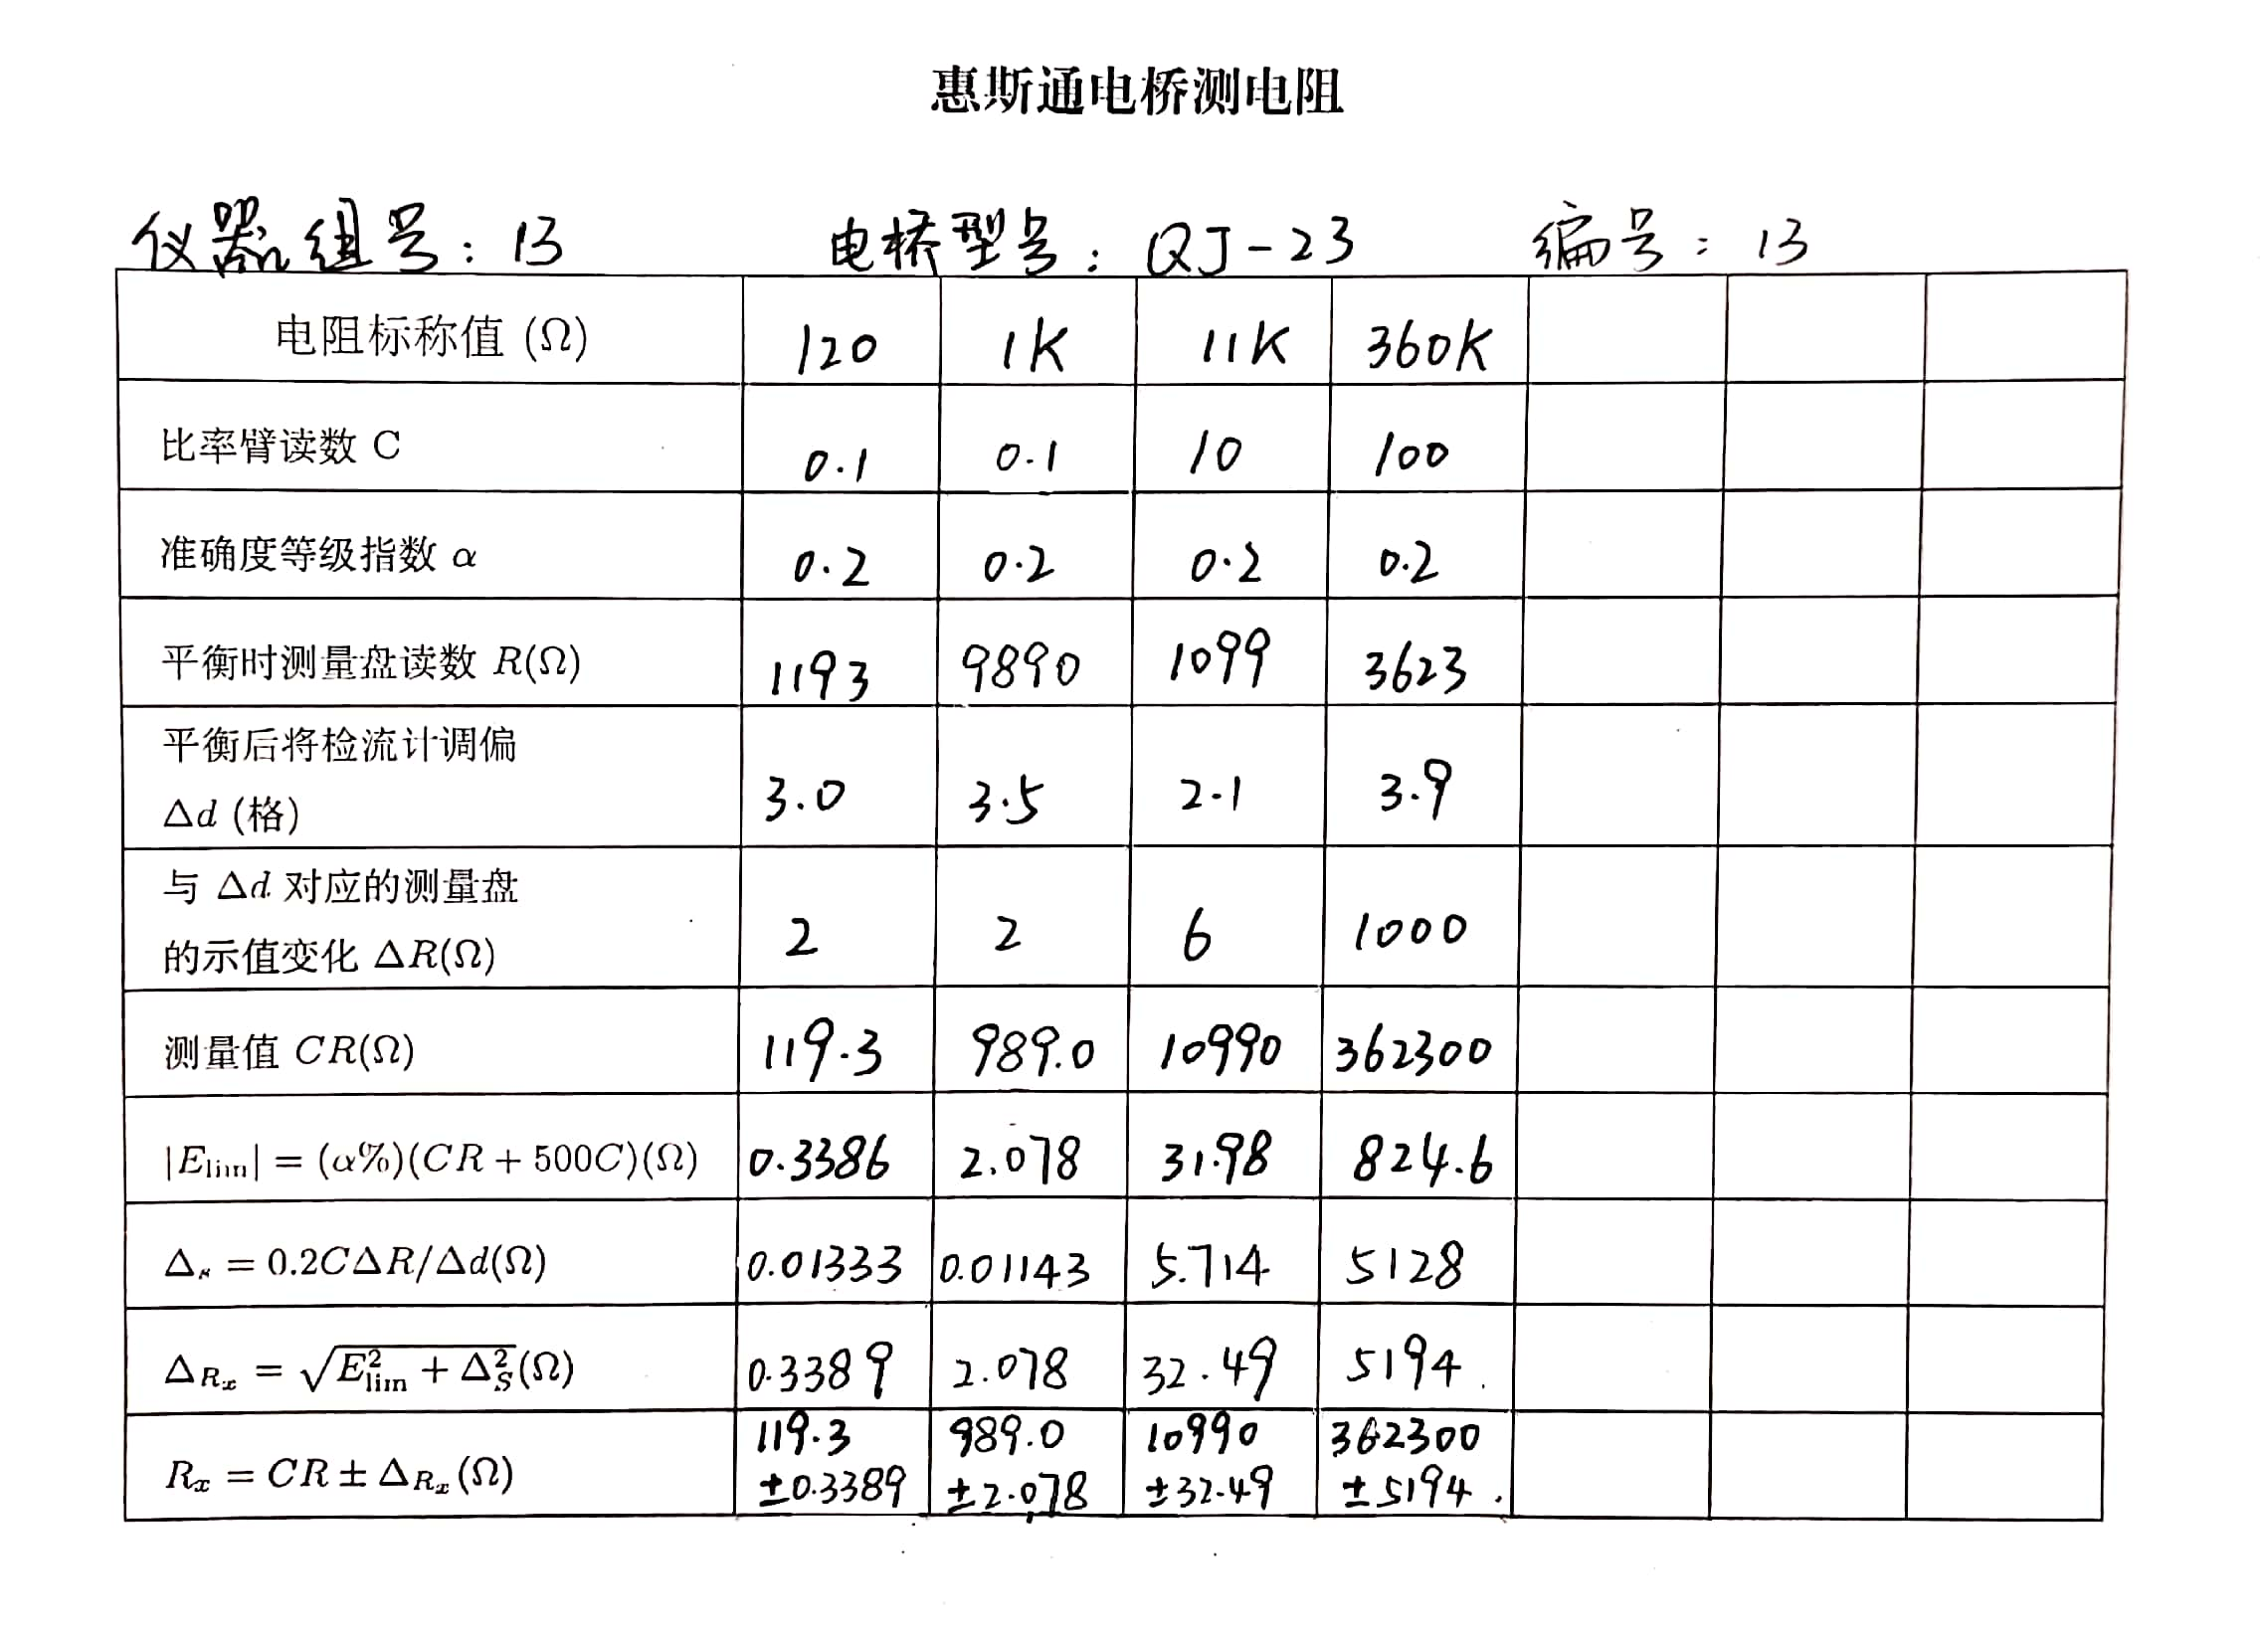
\includegraphics[scale=0.15]{惠斯通电桥测电阻.jpg}
\end{figure}
\begin{figure}[ht]
    \centering
    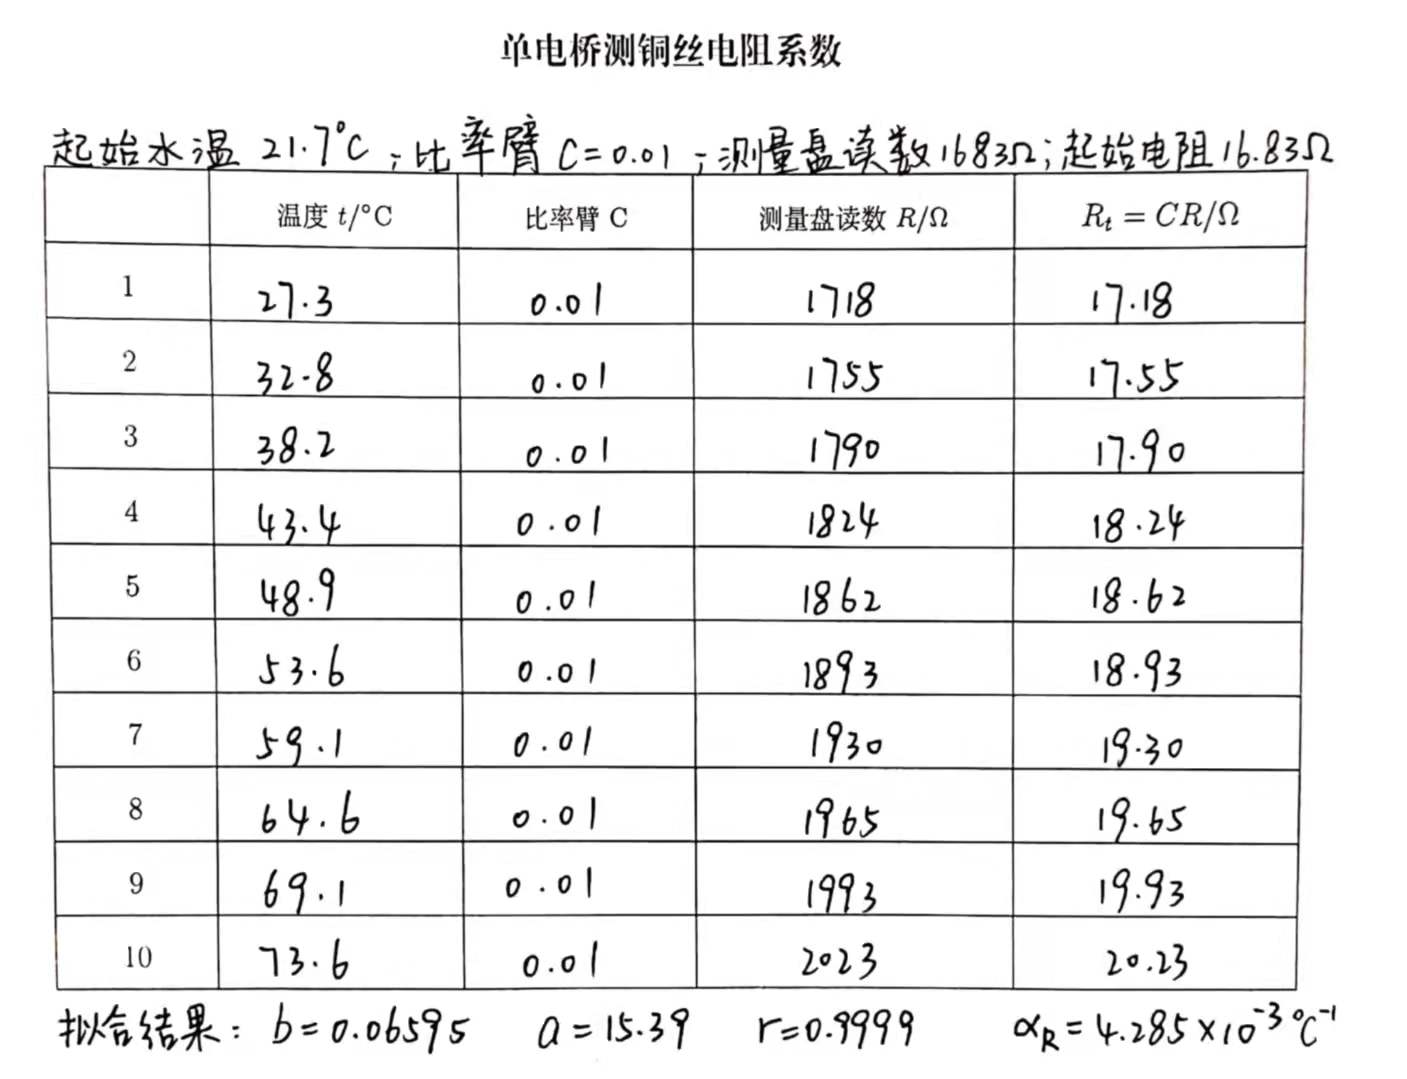
\includegraphics[scale=0.225]{单电桥测铜丝电阻系数.jpg}
\end{figure}
\begin{figure}[ht]
    \centering
    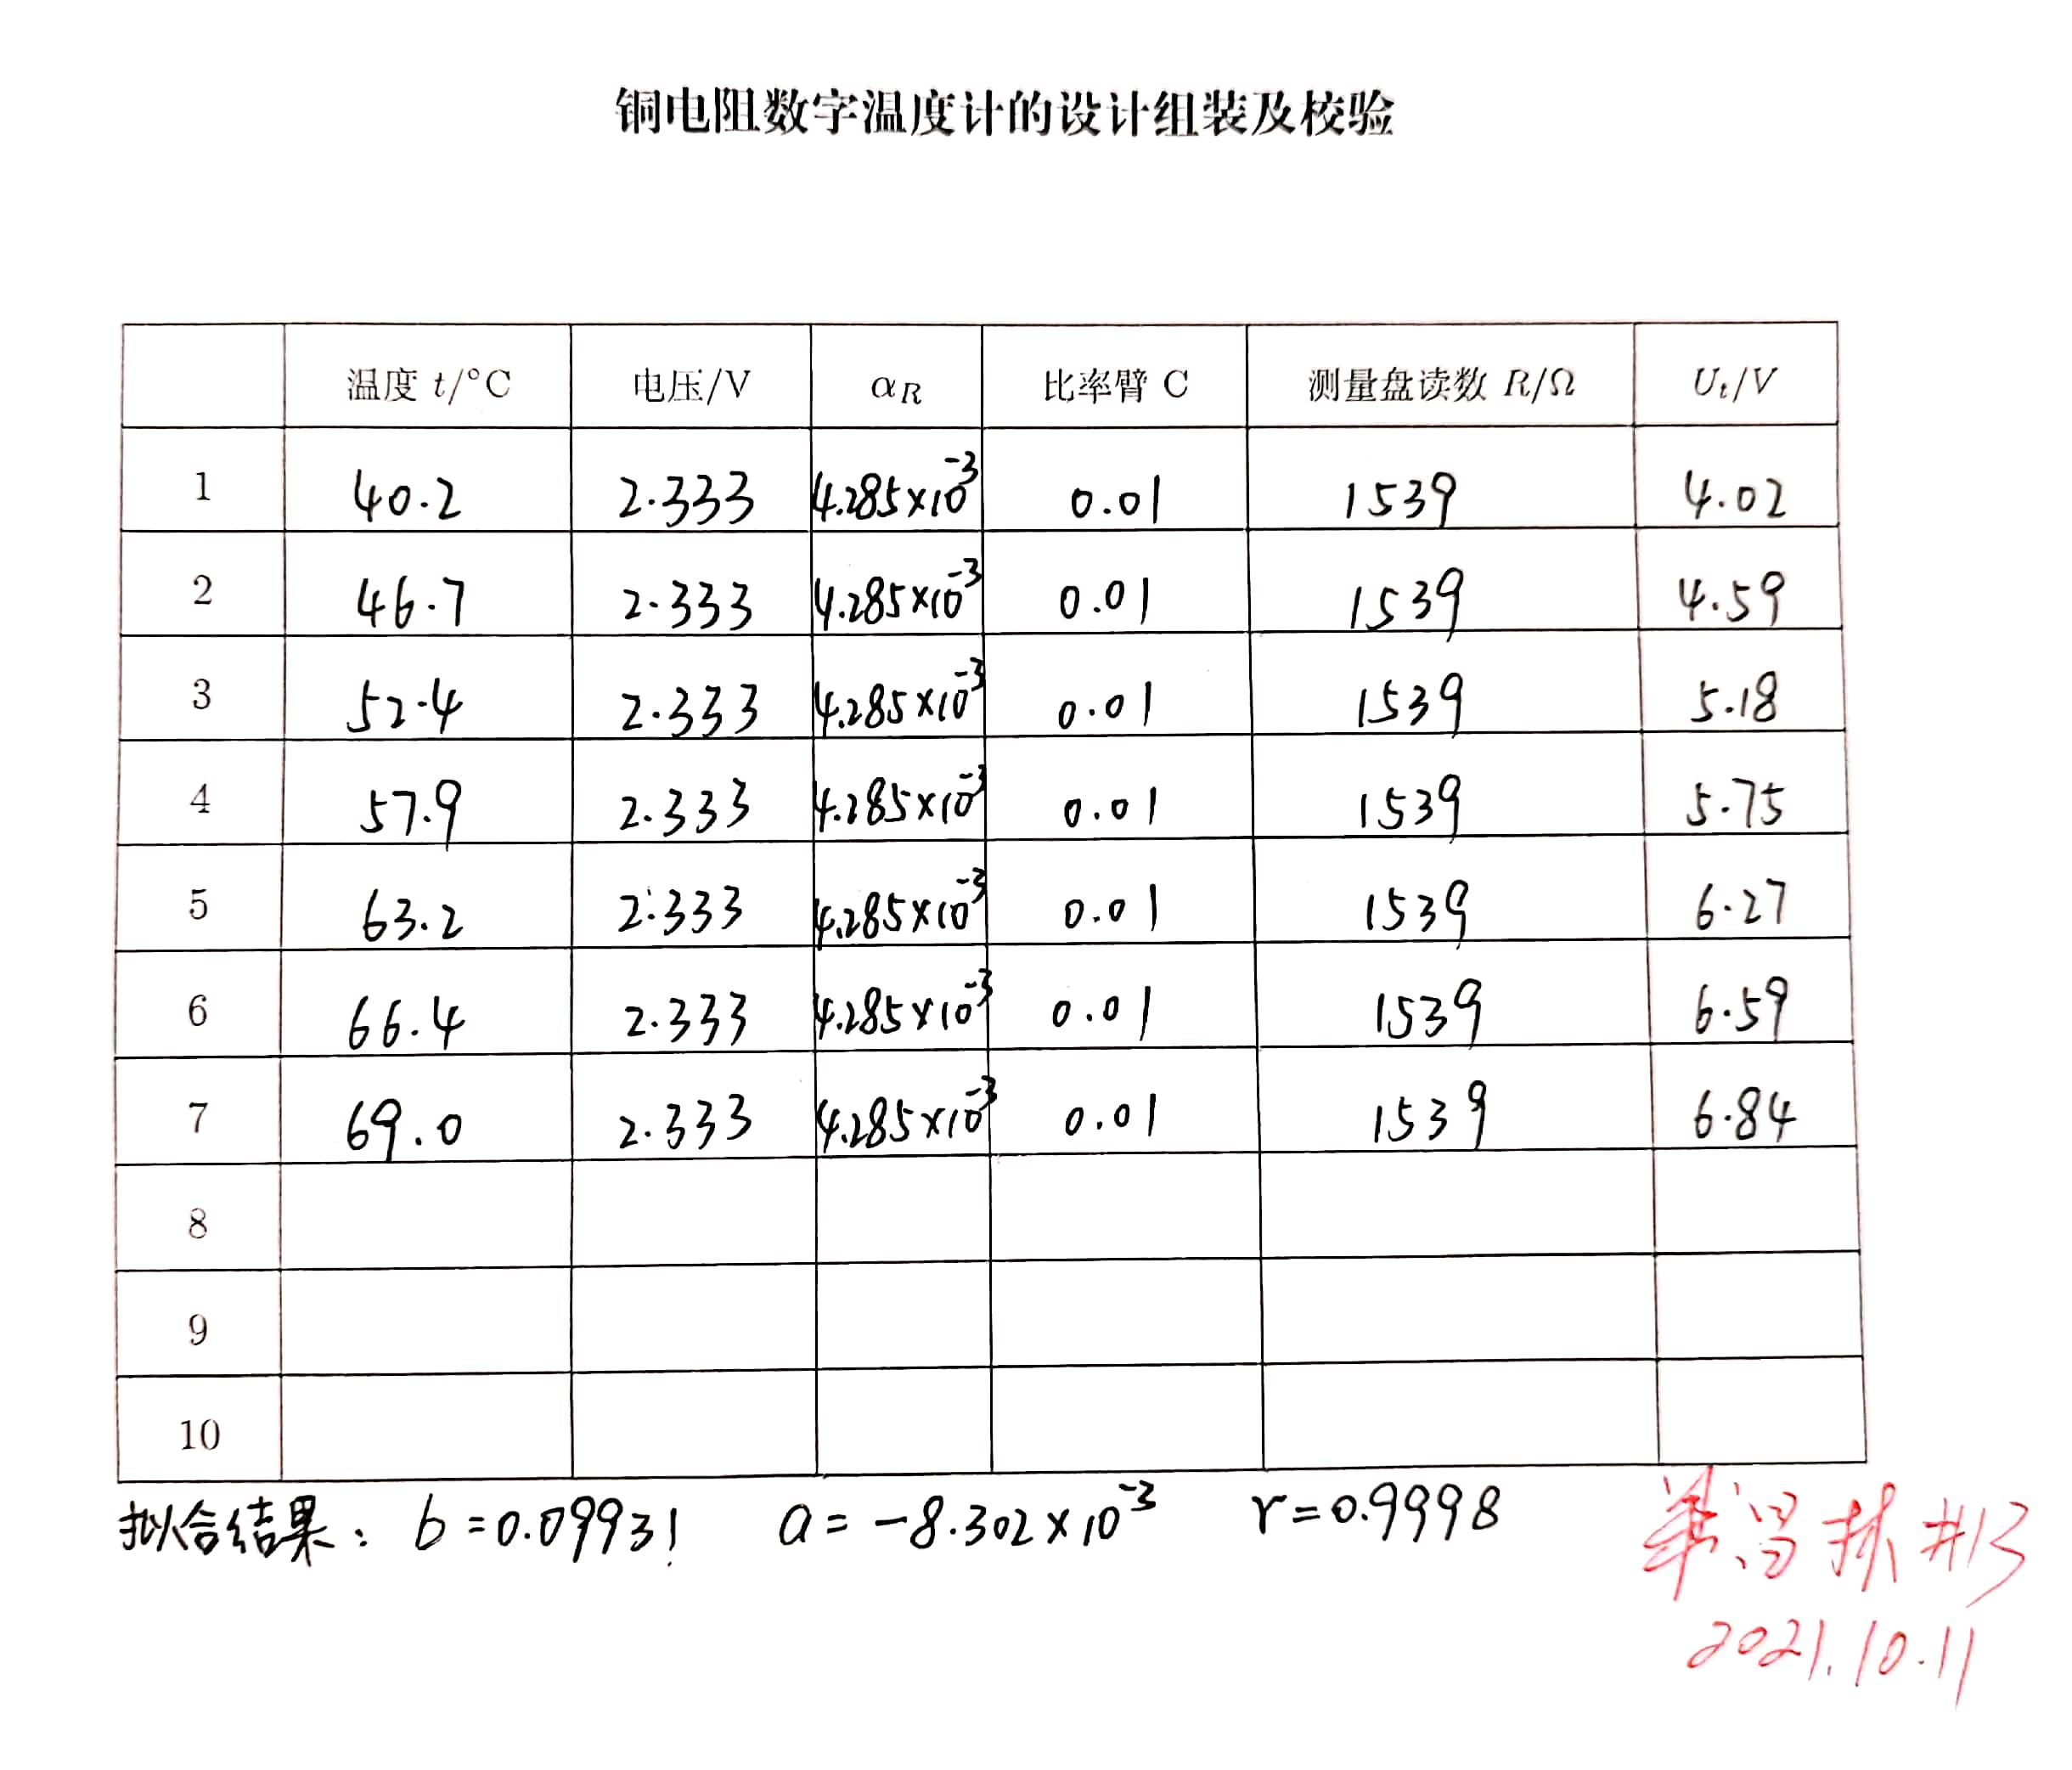
\includegraphics[scale=0.16]{铜电阻数字温度计的设计组装及校验.jpg}

\end{figure}



\end{document}